\documentclass{article}

%packages
\usepackage[LGR]{fontenc}
\usepackage[english,greek]{babel}
\usepackage{amsfonts}
\usepackage{mathtools}
\usepackage{pifont}
\usepackage{amsmath}
\usepackage{algorithm2e}
\usepackage{graphicx}
\usepackage{polynom}


%commands
\newcommand{\blank}[1]{\hspace*{#1}}
\newcommand{\myspace}{\blank{0.3cm}}
\newcommand{\lt}[1]{\latintext #1\greektext}
\newcommand{\gt}[1]{\greektext #1\latintext}
\newcommand{\task}[2]{\newpage\section*{Άσκηση #1:\\#2}}
\newcommand{\blt}[1]{\lt{\textbf{#1}}}
\newcommand{\mymod}[2]{#1 \myspace mod \myspace #2}
\newcommand{\binomialsum}[3]{\sum_{k=#1}^{#2}\binom{#2}{k}(#3)^k}
\newcommand{\myxmark}{\ding{55}}
\newcommand{\myceil}[1]{\left \lceil #1 \right \rceil}
\newcommand{\myfloor}[1]{\left \lfloor #1 \right \rfloor}

%default parameters
\setcounter{MaxMatrixCols}{20}
\setlength{\parindent}{0pt}
\SetKwFor{RepTimes}{repeat}{times}{end}
\SetKwFor{ElifEnd}{else if}{then}{end}

%header
\title{\textbf{\huge \lt{Project II}\\ Κρυπτογραφία Δημοσίου Κλειδιού}}
\author{\LARGE Ασημάκης Κύδρος \\ \LARGE ΑΕΜ: 3881 \\ \LARGE \lt{asimakis@csd.auth.gr}}
\date{\LARGE \today}

\begin{document}
\maketitle
\Large

\task{1}{
    Εφαρμόστε το πρωτόκολλο ανταλλαγής \lt{Diffie-Hellman} για $g = 3, p = 101, a = 77, b = 91$. Υπολογίστε, δηλαδή, το κοινό κλειδί. Υλοποιείστε τον αλγόριθμο γρήγορης ύψωσης σε δύναμη για να το πετύχετε. 
}
{
    Η \lt{Alice} και ο \lt{Bob} έχουν συμφωνήσει στους αριθμούς $g = 3, p = 101$. Επιλέγουν μυστικά κλειδιά 77 και 91 αντιστοίχως και δημοσιεύουν τα $3^{77}, 3^{91}$ αντιστοίχως. Επομένως και οι δύο καταλήγουν στο κοινό κλειδί 
    
    \begin{center}
        $K = \mymod{(3^{77})^{91}}{101} = \mymod{(3^{91})^{77}}{101} \Rightarrow$\\
        $K = 66$
    \end{center}
    
    Το παραπάνω σκηνικό υλοποιείται στο \lt{task 1.py}. Για την γρήγορη ύψωση σε δύναμη χρησιμοποιείται η συνάρτηση \blt{mod\_pow} που ορίζεται στο \lt{myfuncs.py} και ακολουθεί πιστά τον ψευδοκώδικα των σημειώσεων.
}

\task{2}{
    Υλοποιείστε τον αλγόριθμο της γρήγορης ύψωσης σε δύναμη και χρησιμοποιείστε τον για να υπολογίσετε το $\mymod{5^{77}}{19}$.
}
{
    Όπως και στην προηγούμενη άσκηση, ο αλγόριθμος ορίζεται στο \lt{myfuncs.py}. Τρέχοντας το τεστ του \lt{task 2.py} βλέπουμε πως
    
    \begin{equation*}
        \mymod{5^{77}}{19} = 9
    \end{equation*}
    
    Η αποτελεσματικότητα αυτού του αλγορίθμου υπογραμμίζεται με την αστραπιαία ταχύτητα που υπολογίζει τόσο μεγάλα (και ακόμα μεγαλύτερα) εκθετικά.
}

\task{3}{
    Να αποδείξετε ότι ο \lt{n}--οστός πρώτος $p_n$ ικανοποιεί την ανισότητα
    $p_n < 2^{2^n}$
}
{
    Γνωρίζουμε πως 
    \[p_{n + j} < p_1p_2\ldots p_n + 1 \text{ για $j > 0$}\]
    άρα
    \begin{equation}
        p_{n + 1} \leq p_1p_2\ldots p_n + 1  
    \end{equation}
    Θα αποδείξουμε το ζητούμενο με επαγωγή. Παρατηρούμε πως για $n = 1$ ισχύει:
    \[p_1 = 2 < 2^{2^1} \Rightarrow^? 2 < 4 \myspace \checkmark\]
    Έστω ότι ισχύει για τυχαίο $n$. Θα αποδείξουμε ότι ισχύει και για $n + 1$. Εφαρμόζοντας την υπόθεση στην (1) έχουμε:
    \begin{align*}
        p_{n + 1} &\leq p_1p_2\ldots p_n + 1  \Rightarrow\\
        p_{n + 1} &\leq 2^{2^1}2^{2^2}\ldots2^{2^n} + 1 \Rightarrow\\
        p_{n + 1} &\leq 2^{2 + 4 + \ldots + 2^n} + 1 \Rightarrow\\
        p_{n + 1} &\leq 2^{2(1 + 2 + \ldots + 2^{n - 1})} + 1
    \end{align*}
    Είναι γνωστό πως
    \[1 + 2 + 4 + \ldots + 2^{n - 1} = 2^n - 1\]
    άρα
    \begin{align*}
        p_{n + 1} &\leq 2^{2(2^n - 1)} + 1 \Rightarrow\\
        p_{n + 1} &\leq 2^{2^{n + 1} - 2} + 1
    \end{align*}
    Επίσης παρατηρούμε πως
    \[1 < 3\cdot2^{2^{n + 1} - 2} \myspace \forall n > 0\]
    επομένως
    \begin{align*}
        p_{n + 1} &< 4\cdot2^{2^{n + 1} - 2} \Rightarrow\\
        p_{n + 1} &< 2^{2^{n + 1}} \myspace \checkmark
    \end{align*}
    Άρα τελικά όντως ισχύει $p_n < 2^{2^n} \myspace \forall n > 0$
}

\task{4}{
    Έστω \lt{a, b} θετικοί ακέραιοι. Αν $gcd(a,b) = 1$, τότε δείξτε ότι:
    \begin{enumerate}
        \item $gcd(ac, b) = gcd(c, b) \myspace \forall c \in \mathbb{Z}$
        \item $gcd(a + b, a - b) \in \{1, 2\}$ και συγκεκριμένα ότι είναι 2 αν \lt{a, b} περιττοί.
        \item $gcd(2^a - 1, 2^b - 1) = 1$
        \item $gcd(M_p, M_q) = 1$ όπου $M_p = 2^p - 1$ \lt{Mersenne} πρώτοι $(p \not= q)$.
    \end{enumerate}
}
{
    \begin{enumerate}
        \item Έστω $gcd(ac, b) = d_1$. Άρα ισχύει ότι
              \[d_1 | ac, \myspace d_1 | b\]
              Εφόσον $gcd(a, b) = 1$, πηγάζουμε από τα παραπάνω πως
              \[d_1\not| a, d_1 | c\]
              Έστω τώρα ότι το $d_1 \not= gcd(c, b)$, άρα
              \[gcd(c, b) = d_2 > d_1\]
              άρα έχουμε πως
              \[d_2 | c, d_2 | b \Rightarrow d_2 | ac + b\]
              (ο ΚΔ δύο ακεραίων διαιρεί και κάθε γραμμικό συνδυασμό τους).
              Εφόσον όμως $d_2 > d_1$ (εξορισμού) τότε έχουμε πως τελικά
              \[gcd(ac, b) = d_2\]
              και άρα
              \[gcd(ac, b) = gcd(c, b)\]
            
        \item Έστω $gcd(a + b, a - b) = d$. Εφόσον το $d$ διαιρεί τα $a + b, a - b$, θα        διαιρεί και το άθροισμα και τη διαφορά τους. Συγκεκριμένα, έστω
            \[a + b = c_1d, \myspace a - b = c_2d\]
            για αυθαίρετα $c_1, c_2$.\\
            
            Τότε:
            \[(a+b) + (a - b) = c_1d + c_2d \Rightarrow 2a = (c_1 + c_2)d\]
            \[(a+b) - (a - b) = c_1d - c_2d \Rightarrow 2b = (c_1 - c_2)d\]
            Άρα ισχύει 
            \[d | 2a, \myspace d| 2b\]
            και επειδή $gcd(a, b) = 1$ πρέπει
            \[d | 2 \Rightarrow d = \{1, 2\}\]
        
            Έστω ότι τώρα $a, b$ είναι επιπλέον περιττοί, μπορούμε δηλαδή να τους γράψουμε
            \[a = 2k_1 + 1, \myspace b = 2k_2 + 1, \myspace k_1,k_2\in\mathbb{Z}\]
            Άρα
            \[a + b = 2k_1 + 1 + 2k_2 + 1 = 2k_1 + 2k_2 + 2 = 2(k_1 + k_2 + 1) = 2m\]
            \[a - b = 2k_1 + 1 - 2k_2 - 1 = 2k_1 - 2k_2 = 2(k_1 - k_2) = 2n, \myspace m,n\in\mathbb{Z}\]
            Είναι και τα δύο άρτιοι, άρα $2 | (a+b), \myspace 2 | (a-b)$ και επομένως
            \[gcd(a + b, a - b) = 2\]
        \item Έστω $gcd(2^a - 1, 2^b - 1) = d$, και επειδή $gcd(a, b) = 1$ τότε από την        ταυτότητα \lt{Bezout}:
            \[\exists x,y \in\mathbb{Z}\ni ax + by = 1\]
            επίσης
            \[2^a - 1 = c_1d \Rightarrow 2^a = c_1d + 1\]
            \[2^b - 1 = c_2d \Rightarrow 2^b = c_2d + 1\]
            για αυθαίρετα $c_1, c_2$.\\
        
            Τότε:
            \[2^1 = 2^{ax + by} = {2^a}^x{2^b}^y = (c_1d + 1)^x(c_2d + 1)^y\]
        
            Χρησιμοποιούμε την \textbf{διωνυμική ταυτότητα} για να υπολογίσουμε τις προκύπτουσες δυνάμεις:
            \begin{align*}
                  2^1 = &\binomialsum{0}{x}{c_1d}\cdot\binomialsum{0}{y}{c_2d} \Rightarrow \\ 
                  2^1 = (&\binomialsum{1}{x}{c_1d} + 1)(\binomialsum{1}{y}{c_2d} + 1) \Rightarrow\\
                  2^1 = &\binomialsum{1}{x}{c_1d}\cdot\binomialsum{1}{y}{c_2d} +\\
                        &\binomialsum{1}{x}{c_1d} + \binomialsum{1}{y}{c_2d} + 1
            \end{align*}
            Κάθε άθροισμα είναι ένας γραμμικός συνδυασμός των δυνάμεων του $d$ ξεκινώντας από την πρώτη δύναμη.
            Άρα, στην τελική σχέση, ο πρώτος όρος θα έχει κοινό παράγοντα το $d^2$ και οι άλλοι δύο το $d$.
            
            Επομένως, για ακεραίους $m, n, l, k, g$ καταλήγουμε στο
            \[2^1 = d^2\cdot m + d\cdot n + d\cdot l + 1 = d(k + n + l) + 1 \Rightarrow\]
            \[1 = d\cdot g\]
            Άρα ισχύει $d | 1$ και άρα το $d = 1$ ($d, g$ θετικά).
        \item Εφόσον $p \not= q$ τότε $gcd(p, q) = 1$ και άρα ισχύει το ζητούμενο με            εφαρμογή του από πάνω. 
    \end{enumerate}
}

\task{5}{
    Έστω $a,b,c\in\mathbb{Z}$ και $\delta = a^2 - 4bc^2 \not= 0$. Δείξτε ότι το $gcd(\delta, 4c^2)$ είναι τετράγωνο.
}
{
    Ισχύει γενικά πως
    \[gcd(a^n, b^n) = [gcd(a, b)]^n, \myspace \forall a,b\in\mathbb{Z}\]
    Αυτό φαίνεται από τις πρωτογενείς αναλύσεις των $a, b$:
    \begin{align*}
        a &= p_1^{e_{11}}p_2^{e_{12}}p_3^{e_{13}}\ldots\\
        b &= p_1^{e_{21}}p_2^{e_{22}}p_3^{e_{23}}\ldots
    \end{align*}
    \begin{equation}
        \Rightarrow gcd(a, b) = p_1^{min(e_{11}, e_{21})}p_2^{min(e_{12}, e_{22})}p_3^{min(e_{13}, e_{23})}\ldots
    \end{equation}
    Υψώνοντας σε κοινή δύναμη έχουμε:
    \begin{align*}
        a^n &= (p_1^{e_{11}}p_2^{e_{12}}p_3^{e_{13}}\ldots)^n
            = p_1^{ne_{11}}p_2^{ne_{12}}p_3^{ne_{13}}\ldots\\
        b^n &= (p_1^{e_{21}}p_2^{e_{22}}p_3^{e_{23}}\ldots)^n
            = p_1^{ne_{21}}p_2^{ne_{22}}p_3^{ne_{23}}\ldots
    \end{align*}
    \begin{align*}
        \Rightarrow gcd(a^n, b^n) &= p_1^{min(ne_{11}, ne_{21})}p_2^{min(ne_{12}, ne_{22})}p_3^{min(ne_{13}, ne_{23})}\ldots\\
            &= p_1^{n\cdot min(e_{11}, e_{21})}p_2^{n\cdot min(e_{12}, e_{22})}p_3^{n\cdot min(e_{13}, e_{23})}\ldots\\
            &= (p_1^{min(e_{11}, e_{21})}p_2^{min(e_{12}, e_{22})}p_3^{min(e_{13}, e_{23})}\ldots)^n
    \end{align*}
    \begin{equation*}
        (2)\Rightarrow gcd(a^n, b^n) = [gcd(a, b)]^n \myspace \checkmark
    \end{equation*}

    Είναι επίσης τετριμμένο πως 
    \[gcd(a + mb, b) = gcd(a, b), \myspace \forall a,b,m\in\mathbb{Z}\]
    
    Γνωρίζοντας τα παραπάνω, έχουμε:
    \begin{align*}
        gcd(a, 2c) = d &\Rightarrow gcd(a^2, 4c^2) = d^2 \land d^2 | a^2 - 4bc^2\\
        &\Rightarrow gcd(\delta, 4c^2) = d^2 \myspace \square
    \end{align*}
}

\task{6}{
    Επαληθεύστε πειραματικά ότι για όλους τους περιττούς ακεραίους $< 2^{20}$ ισχύει \[\frac{\sigma(n)}{n} < \frac{e^\gamma}{2}ln(ln(n)) + \frac{0.74}{ln(ln(n))}\]
    όπου $\gamma$ η σταθερά \lt{Euler}.
}
{
    Αρχικά αναδιαμορφώνουμε την ανισότητα ώστε να μεγιστοιποιήσουμε την ταχύτητα υπολογισμού και, κατ' επέκταση, επαλήθευσής της:
    \begin{align*}
        \frac{\sigma(n)}{n} &< \frac{e^\gamma}{2}ln(ln(n)) + \frac{0.74}{ln(ln(n))}\\
        \xRightarrow{\cdot nln(ln(n))} \sigma(n)ln(ln(n)) &< \frac{e^\gamma}{2}nln^2(ln(n)) + 0.74n\\
        \Rightarrow \sigma(n)ln(ln(n)) &< n(\frac{e^\gamma}{2}ln^2(ln(n)) + 0.74)\\
        \xRightarrow[\mathcal{L} = ln(ln(n))]{\mathcal{C}_e = \frac{e^\gamma}{2}} \sigma(n)\mathcal{L} &< n(\mathcal{C}_e\mathcal{L}^2 + 0.74)
    \end{align*}
    
    Τώρα μπορούμε να δοκιμάσουμε την ανισότητα στο δεδομένο πεδίο ορισμού. Τρέχοντας το \lt{task 6.py} αποβραδίς ανακαλύπτουμε πως η ανισότητα όντως ισχύει για κάθε περιττό ακέραιο $<2^{20}$. 
}

\task{7}{
    Αποδείξτε ότι οι αριθμοί
    \[9999109081, 6553130926752006031481761 \]
    είναι \lt{Carmichael}. Μπορείτε να βρείτε κάποιον μεγαλύτερο?
}
{
    Αριθμοί \lt{Carmichael} λέγονται οι ψευδοπρώτοι αριθμοί,\\ δηλαδή εκείνοι οι σύνθετοι περιττοί που περνούν το τεστ του \lt{Fermat}.\\
    Μπορούμε να εκφράσουμε το παραπάνω με μαθηματικά ως
    \begin{center}
        $n: \myspace \text{\lt{Carmichael}}$\\
        $\iff$\\
        $\forall a\in(1, n)\cap\mathbb{Z} \ni gcd(a, n) = 1 \implies a^{n-1} \equiv 1 (\text{\lt{mod n}})$
    \end{center}
    
    Υλοποιούμε επομένως πρόγραμμα που πιστοποιεί την ιδιότητα \lt{Carmichael} ελέγχοντας το παραπάνω $\forall a\in[2, n - 1]$.
    Ο έλεγχος του \lt{task 7.py} επαληθεύει ότι οι δωσμένοι αριθμοί είναι όντως
    \lt{Carmichael}. \\
    
    Παρόλο που δεν έχει αποδειχθεί, οι \lt{Carmichael} φαίνονται αρκετά σπάνιοι, και δεν υπάρχει κάποιος τύπος ή μέθοδος για την εύρεσή τους. Για να βρούμε κάποιον μεγαλύτερο, επομένως, μπορούμε μόνο να ψάξουμε τυφλά πέρα από τον
    6553130926752006031481761 για περιττούς που\\ ικανοποιούν το παραπάνω κριτήριο.\\
    Η \lt{Monte Carlo} εκδοχή του προηγουμένου αλγορίθμου δίνει τον
    \[6553130926752006031481777\]
    ως τον επόμενο \lt{Carmichael}, προφανώς με κάποια\\ πιθανότητα.
}

\task{8}{
    Ελέγξτε αν το ζεύγος $835335\cdot2^{39014} \pm 1$ ικανοποιεί το τεστ του \lt{Fermat}.
}
{
    Στο \lt{task 8.py} υλοποιείται το τεστ του \lt{Fermat}, και ακολουθεί πιστά την θεωρία. Τρέχοντας το τεστ για το ζεύγος βλέπουμε πως είναι και οι δύο ψευδοπρώτοι.\\
    
    Μαζί παρέχεται και η \lt{Monte Carlo} εκδοχή του τεστ του \lt{Fermat}. Ενώ το αποτέλεσμα αυτής θα είναι πολύ πιο έμπιστο, εφόσον τρέχουμε το απλό τεστ για πολλούς τυχαίους αριθμούς, η μέθοδος είναι κλάσεις πιο αργή.
}

\task{9}{
    Υλοποιείστε τον αλγόριθμο της δοκιμαστικής διαίρεσης και χρησιμοποιείστε τον για να\\ παραγοντοποιείσετε τους $n_1 = 2^{62} - 1, n_2 = 2^{102} - 1$.
}
{
    Η δοκιμαστική διαίρεση υλοποιείται στο \lt{myfuncs.py}, για λόγους επαναχρησιμοποίησης σε επόμενες ασκήσεις. Η υλοποίησή του δεν παρεκκλίνει από τον ψευδοκώδικα των σημειώσεων.\\
    
    Η αποτελεσματικότητά του γίνεται φανερή στην παραγοντοποίηση των δωσμένων αριθμών, καθώς επιστρέφει
    \begin{center}
        $[3, 715827883, 2147483647]_{n_1}$\\
        
        $[3, 3, 7, 103, 307, 2143, 2857, 6529, 11119, 43691, 131071]_{n_2}$
    \end{center}
    με ικανοποιητική ταχύτητα.
}

\task{10}{
    Υλοποιήστε τον αλγόριθμο του \lt{Lehman} για παραγοντοποίηση και βρείτε το ποσοστό επιτυχίας για 1000 επαναλήψεις του παρακάτω πειράματος:\\
    \textit{Έστω τυχαίος περιττός \lt{100-bit} ακέραιος. Αν ο αλγόριθμος του \lt{Lehman} τον παραγοντοποιήσει μέσα σε 10 δευτερόλεπτα, θεωρούμε επιτυχία.}
}
{
    Υλοποιούμε τον αλγόριθμο του \lt{Lehman} βασιζόμενοι στον ψευδοκώδικα της θεωρίας. Πρόκειται για υπολογιστικά\\ βαρύ αλγόριθμο, οπότε αξίζει να κάνουμε όσες τροποποιήσεις μπορούμε για να τον επιταχύνουμε.\\
    
    Από άποψη υλοποίησης, πρέπει να ελαχιστοποιήσουμε τις απαιτούμενες ρίζες και να ανακυκλώσουμε όσες το δυνατόν περισσότερες τιμές γίνεται. Ας δούμε το πεδίο ορισμού του $\alpha$:
    \begin{equation*}
        \myceil{\sqrt{4kn}} \leq \alpha \leq \myfloor{\sqrt{4kn} + \frac{n^{1/6}}{4\sqrt{k}}}
    \end{equation*}
    Έχουμε 3 ρίζες να υπολογίσουμε μόνο γι αυτό το κομμάτι. Όμως, το $4\sqrt{k}$ μοιάζει με το $\sqrt{4kn}$. Αν το φέρουμε στην ίδια μορφή, έχουμε:
    \begin{align*}
        \myceil{\sqrt{4kn}} \leq \alpha &\leq \myfloor{\sqrt{4kn} + \frac{n^{1/6}n^{1/2}}{4\sqrt{k}\sqrt{n}}} \Rightarrow\\
        \myceil{\sqrt{4kn}} \leq \alpha &\leq \myfloor{\sqrt{4kn} + \frac{n^{2/3}}{4\sqrt{kn}}} \Rightarrow\\
        \myceil{\sqrt{4kn}} \leq \alpha &\leq \myfloor{\sqrt{4kn} + \frac{(\sqrt[3]{n})^2}{2\sqrt{4kn}}}
    \end{align*}
    και κάνοντας ομώνυμα κλάσματα έχουμε
    \begin{align*}
        \myceil{\sqrt{4kn}} \leq \alpha &\leq \myfloor{\frac{2\cdot4kn + (\sqrt[3]{n})^2}{2\sqrt{4kn}}} \Rightarrow\\
        \myceil{\sqrt{4kn}} \leq \alpha &\leq \myfloor{\frac{4kn + 0.5(\sqrt[3]{n})^2}{\sqrt{4kn}}}
    \end{align*}
    Καταφέραμε, λοιπόν, να διώξουμε την έκτη ρίζα του $n$, να ανακυκλώσουμε τις τιμές $\sqrt{4kn}$, $\sqrt[3]{n}$ και $4kn$, που επανεμφανίζονται, και να μειώσουμε το πλήθος των απαιτούμενων ριζών προς υπολογισμό σε \textit{όλο τον κώδικα} σε 3.\\
    
    Όσο αφορά την εκτέλεση, μας νοιάζει μόνο αν ο αλγόριθμος τερματίζει σε 10 δευτερόλεπτα, και όχι το αποτέλεσμά του. Επομένως, αν ξεπεραστεί αυτό το χρονικό περιθώριο, δεν έχει νόημα να περιμένουμε και μπορούμε να το τερματίσουμε νωρίς. Γι αυτό το λόγο τρέχουμε το κάθε τεστ σε ένα νήμα και το ''σκοτώνουμε'' αν περάσουν 10 δεύτερα.\\
    
    Τα παραπάνω υλοποιούνται στο \lt{task 10.py}. Για τις 1000 επαναλήψεις του πειράματος ο αλγόριθμος σκοράρει \textbf{18.9\%}. Λαμβάνοντας υπόψιν το γεγονός πως 10 δευτερόλεπτα είναι άκρως μη αντιπροσωπευτικό ταβάνι για αξιολόγηση αλγορίθμου παραγοντοποίησης, το αποτέλεσμα αυτό είναι αρκετά καλό.\\

    Διπλασιάζοντας το ταβάνι χρόνου, το ποσοστό επιτυχίας ανεβαίνει στο \textbf{20.6\%}. Βλέπουμε πως, ακόμα και για τις ακραίες μας απαιτήσεις χρόνου, ο αλγόριθμος του \lt{lehman} καταφέρνει να παραγοντοποιήσει το 1/5 των δειγμάτων.
}

\task{11}{
    Χρησιμοποιείστε τον αλγόριθμο του \lt{Pollard} σε συνδυασμό με τον αλγόριθμο του \lt{Floyd} για να παραγοντοποιείσετε τον $N = 2^{257} - 1$.
    Υποθέστε $F(X) = (X^2 + 1)\text{\lt{ mod} $N$}$ με έλεγχο
    \[1 < gcd(|X - Y|, N) < N\]
}
{
    Ο αλγόριθμος υλοποιείται στο \lt{task 11.py}. Αποτελεί απλή παραλλαγή του παραδοσιακού αλγορίθμου του \lt{Floyd} με τις αλλαγές που μας δώθηκαν. Ο αλγόριθμος αυτός χρησιμοποιεί το γεγονός ότι τα \lt{collisions} σε μεγάλο δακτύλιο δεν είναι και τόσο συχνά, για να ''μαντέψει'' παράγοντες του αριθμού που δεν είναι προφανείς. Πράγματι, όσο πλησιάζουμε σε διένεξη, προσεγγίζουμε έναν \lt{trivial factor}. Αν $x = y$, τότε $gcd(|x - y|, N) = N$, ενώ αν $|x - y| = 1$ τότε $gcd(|x - y|, N) = 1$.\\
    
    Η μέθοδος είναι αρκετά αποτελεσματική. Έπειτα από ανεκτό χρονικό διάστημα, επιστρέφει τον (μικρό) παράγοντα
    \begin{equation*}
        \approx 5.8688966023081812065445\cdot10^{67}\\
    \end{equation*}
    Το ακριβές νούμερο μπορεί να βρεθεί στο προαναφερόμενο αρχείο.
}

\task{12}{
    Με \lt{RSA public key} $(N, e) = (11413, 19)$\\ αποκρυπτογραφήστε το μήνυμα
    \begin{center}
        \lt{C} = (3203, 909, 3143, 5255, 5343, 3203, 909, 9958, 5278, 5343, 9958, 5278, 4674, 909, 9958, 792, 909, 4132, 3143, 9958, 3203, 5343, 792, 3143, 4443)
    \end{center}
}
{
    Εφόσον γνωρίζουμε το $N$ μπορούμε βρούμε την παραγοντοποίησή του. Το πράττουμε αυτό χρησιμοποιώντας τον αλγόριθμο της δοκιμαστικής διαίρεσης από πριν.\\
    
    Έχοντας τους παράγοντες του $N$, υπολογίζουμε το $\phi(N)$, με βάση τον τύπο
    \begin{equation*}
        \phi(N) = N(1 - \frac{1}{p})(1 - \frac{1}{q})
    \end{equation*}
    όπου $p, q$ οι παράγοντες του N (εξ' ορισμού 2 μεγάλοι διαφορετικοί πρώτοι αριθμοί).\\
    
    Τώρα έχουμε όλα τα εργαλεία για να κάνουμε \lt{brute force} το μυστικό κλειδί $d$, δοκιμάζοντας την παρακάτω ισότητα:
    \begin{equation*}
        e\cdot d \equiv 1 \text{ \lt{(mod} $\phi(N)$)} \myspace \forall d\in[1,\phi(N))
    \end{equation*}
    
    \newpage
    
    Καταλήγουμε στο $d = 1179$. Πλέον μπορούμε να αποκρυπτογραφήσουμε το \lt{C}, το οποίο κατά τα γνωστά γίνεται\\ υπολογίζοντας το
    \begin{equation*}
        m_i = c_i^d \text{ \lt{(mod $N$)}}
    \end{equation*}
    για κάθε $c_i$ του \lt{C}. Προφανώς χρησιμοποιούμε τον αλγόριθμο της γρήγορης ύψωσης σε δύναμη για να το καταφέρουμε.\\
    
    Τελικά καταλήγουμε στο παρακάτω αποκρυπτογραφημένο μήνυμα:
    \begin{center}
        \lt{\textbf{\textit{welcowe to the real world}}}
    \end{center}
    το οποίο είναι \lt{(typo-d) quote} του \lt{Morpheus} από το\\ \lt{\textit{Matrix}}.\\
    
    Όλη η παραπάνω διαδικασία υλοποιείται στο \lt{task 12.py}.
}

\task{13}{
    Αποκρυπτογραφήστε το μήνυμα που\\ βρίσκεται στο \lt{github}, που κρυπτογραφήθηκε με \lt{textbook-RSA} με \lt{public key}
    \[(N, e) = (194749497518847283, 50736902528669041)\]
    και κατόπιν κωδικοποιήθηκε. Για να βρείτε το \lt{secret key $d$} εφαρμόστε την επίθεση του\\ \lt{Wiener}.
}
{
    Η αποκωδικοποίηση του \lt{string} που υπάρχει στο \lt{github} από \lt{Base64} δίνει ένα μήνυμα \lt{C} σαν και αυτό του δεδομένου της άσκησης 12.\\
    
    Εφαρμόζουμε επίθεση \lt{Wiener} για να βρούμε το μυστικό κλειδί $d$. Για την υλοποίησή του, η οποία βρίσκεται στο \lt{task 13.py}, χρειάστηκε να οριστούν οι συναρτήσεις \blt{continued\_fraction} και \blt{convergent\_ratio}, που υπολογίζουν συνεχές κλάσμα και τον λόγο συκλίνοντος κλάσματος, αντιστοίχως.\\
    
    Από εκεί και πέρα η υλοποίηση της επίθεσης ακολουθεί την θεωρία. Έχοντας το $d$, αποκαλύπτουμε ότι το μήνυμα είναι
    \begin{center}
        \blt{\textit{ Just because you are a character doesn't mean that you have character}}
    \end{center}
    το οποίο είναι \lt{quote} του \lt{Winston Wolf} από την ταινία\\ \lt{\textit{Pulp Fiction}}.
}

\task{14}{
    Έστω το κλειδί μιας \lt{naive} ψηφιακής \lt{RSA} υπογραφής $(N, e) = (899, 839)$. Αν η υπογραφή του μηνύματος $m = 3$ είναι $s = 301$, επαληθεύστε αν η υπογραφή είναι σωστή.
}
{
    Μια ψηφιακή υπογραφή \lt{RSA} κρίνεται σωστή/έγκυρη όταν ισχύει
    \begin{equation*}
        m = s^e \text{ \lt{(mod $N$)}}
    \end{equation*}
    
    Αντικαθιστώντας για τις γνωστές σταθερές βλέπουμε πως
    \begin{center}
        $3 =^? 301^{839} \text{ \lt{(mod 899)}} \Rightarrow$\\
        $3 =^? 675 \text{ \myxmark}$
    \end{center}
    Άρα η υπογραφή δεν είναι σωστή.\\
    
    Το παραπάνω επαληθεύεται στο \lt{task 14.py}. Για την πιστοποίηση χρησιμοποιείται ο αλγόριθμος της γρήγορης ύψωσης σε δύναμη.
}

\task{15}{
    Στείλτε ένα κρυπτογραφημένο μήνυμα στον ιδιοκτήτη του δημοσίου κλειδιού με αναγνωριστικό \lt{0xEB1185F82713D6DF}.
}
{
    Έχοντας εγκατεστημένο το \lt{GPG} στον υπολογιστή μας, παράγουμε κλειδιά μέσω της γραμμής εντολών επικαλώντας το
    \begin{center}
        \blt{gpg --full-gen-key}
    \end{center}
    Συμπληρώνουμε κατά τα γνωστά και πλέον έχουμε το δημόσιο κλειδί μας.\\

    Μετέπειτα εισάγουμε το δημόσιο κλειδί του συγγραφέα, που αντιστοιχίζεται στο δεδομένο αναγνωριστικό. Αυτό γίνεται επικαλώντας
    \begin{center}
        \blt{gpg --import}
    \end{center}
    όπου επικολλάμε ολόκληρο το κλειδί και πατάμε \lt{enter}, \lt{ctrl + z} και \lt{enter}.\\

    Αφού εισάγουμε το δημόσιο κλειδί του παραλήπτη, προχωράμε στην κρυπτογράφηση. Η διαδικασία ξεκινά επικαλώντας
    \begin{center}
        \blt{gpg -a --encrypt --recipient (recipient email)}
    \end{center}
    και δίνοντας το μήνυμα.

    \newpage
    
    Εδώ κρυπτογραφήθηκε το εξής μήνυμα:
    \begin{center}
        \large
        \lt{\textit{A mortal, Frodo, who keeps one of the Great Rings does not die; but he does not grow or obtain more life. He merely continues, until at last every minute is a weariness. And if he often uses the Ring to make himself invisible, he fades; he becomes in the end invisible permanently, and walks in the twilight under the eye of the dark power that rules the Rings.}}
    \end{center}
    το οποίο είναι \lt{quote} του \lt{Gandalf} από το \textit{\lt{Lord of the Rings}}.\\

    Στέλνουμε το κρυπτόγραμμα και το δημόσιο κλειδί μας στον παραλήπτη και μας στέλνει αυτός πίσω ένα δικό του κρυπτόγραμμα. Το αποκρυπτογραφούμε επικαλώντας
    \begin{center}
        \blt{gpg --decrypt}
    \end{center}
    και δίνοντας το κρυπτόγραμμα με τον προαναφερώμενο τρόπο. Ανακαλύπτουμε,
    έτσι, το πιστοποιητικό-\lt{hash}:
    \begin{center}
        \textit{\blt{23c5877aef9705c4d17b88cd59f81f5d}}
    \end{center}
}

\task{\lt{Bonus}}{
    Υλοποιείστε πρόγραμμα που επιστρέφει ασφαλείς πρώτους μήκους \lt{2048 bits} σε περίπου 3 λεπτά.
}
{
    Επιχειρούμε το ζητούμενο έμμεσα αναζητώντας \lt{Sophie Germain} πρώτους μήκους 2047 \lt{bits}. Ο γενικός αλγόριθμος πιστοποίησης \lt{Sophie Germain prime} και άρα \lt{safe prime} είναι:

    \begin{algorithm}
    \Large
        \latintext
        \KwData{$n: \text{ desired bit length}$}
        \KwResult{$p \ni (p, 2p+1) \text{ both prime}$}
        $p \gets \text{random integer of n bits}$\;
        \While{True}{
            \eIf{$p$ and $2p+1$ are both prime}{
                return $p$\;
            }{
                $p \gets p + 2$\;
            }
        }
        \caption{\large Safe prime generator}
    \end{algorithm}

    \newpage

    Άρα σκοπός μας είναι να κάνουμε τον έλεγχο \blt{is\_prime} όσο πιο γρήγορο γίνεται. Το πιο γρήγορο \lt{primality test} βασίζεται στο τεστ των \lt{Miller-Rabin}:

    \begin{algorithm}
        \Large
        \latintext
        \KwData{$n: \text{ integer to be tested}$}
        \KwResult{$Composite \lor Probable\text{ }Prime$}
        $a \gets \text{random integer in } (2, n - 1)$\;
        Find s,d such that $d\cdot 2^s = n - 1$\;
        $b \gets a^d \text{ mod } n$\;
        \If{$b \equiv \pm 1 (\text{mod } n$)}{
            return $Probable\text{ }Prime$\;
        }
        \RepTimes{$s - 1$}{
            $b \gets b^2 \text{ mod }n$\;
            \uIf{$b \equiv 1 (\text{mod }n)$}{
                return $Composite$\;
            }
            \ElseIf{$b = -1 (\text{mod }n)$}{
                return $Probable\text{ }Prime$\;
            }                
        }
        return $Composite$
        \caption{\large Miller-Rabin compositeness test}
    \end{algorithm}

    το οποίο, επειδή είναι πιθανοτικός αλγόριθμος, χρειάζεται να τρέξει πολλαπλές φορές για το ίδιο νούμερο για να γίνει η κρίση $Probable\text{ }Prime$ έμπιστη.\\

    Μπορούμε να βελτιώσουμε την απόδοση αποκλείωντας κάποιους ακεραίους προτού τρέξουμε καν \lt{Miller-Rabin}. Καθώς οι περισσότερες περιπτώσεις έχουν κάποιο μικρό πρώτο ως διαιρέτη, αξίζει να εφαρμόσουμε \blt{trial division} κάθε $n$ για να αποκλείσουμε τις τετριμμένες περιπτώσεις νωρίς.\\

    Βρίσκουμε δυναμικά τους μικρούς πρώτους με το Κόσκινο του Ερατοσθένη. Καθώς ψάχνουμε ασφαλείς πρώτους, μπορούμε να κάνουμε μια περαιτέρω βελτίωση και να εφαρμόσουμε \textit{\lt{Combined Sieve}} στην \lt{trial division}:

    \begin{algorithm}
        \Large
        \latintext
        \KwData{$n: \text{ integer to be tested}$}
        \KwResult{$Composite \lor Probable\text{ }Prime$}
        Find small primes using the sieve of Eratosthenes\;
        \ForAll{small primes s}{
            \If{$n \equiv 0 \lor \frac{s - 1}{2} (\text{mod } s)$}{
                return $Composite$\;
            }
        }
        return $Probable\text{ }Prime$
        \caption{\large Trial Division with combined sieve}
    \end{algorithm}

    Άρα η \lt{is\_prime} γίνεται τελικά:

     \begin{algorithm}
        \Large
        \latintext
        \KwData{$n: \text{ integer to be tested}$}
        \KwResult{$True \lor False$}
        run Trial Division with combined sieve\;
        \If{$Composite$}{
            return $False$
        }
        run Miller-Rabin at least 4 times\;
        \eIf{at least one finds $Composite$}{
            return $False$
        }{
        return $True$
        }
        
        \caption{Fast primality test}
    \end{algorithm}

    Μπορούμε να κάνουμε μια τελευταία βελτίωση στον αρχικό αλγόριθμο. Ισχύει πως
    \lt{\begin{equation*}
        \frac{p-1}{2} \text{ prime} \land 2^{p - 1} \equiv 1 (\text{mod }p) \rightarrow p \text{ prime}
    \end{equation*}}
    άρα αντί να τρέχουμε την \lt{is\_prime} και στο $2p+1$ μπορούμε να κάνουμε ένα απλό \lt{Fermat} τεστ σ' αυτό, με βάση 2.\\

    Όλα τα παραπάνω υλοποιούνται σε \lt{python} στο \lt{safeprimegen.py}. Μέσα του βρίσκονται και πηγές/αποδείξεις. Το \lt{test.py} τρέχει την γεννήτρια 100 φορές και επιστρέφει τα παρακάτω αποτελέσματα:
    \begin{center}
        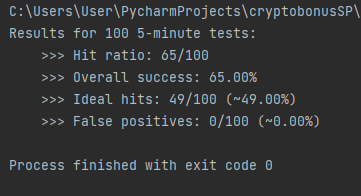
\includegraphics[scale=1]{images/results-sp-test1.png}
    \end{center}

    \lt{Ideal hits} είναι τα τεστ που όντως τελείωνουν μέσα σε 3 λεπτά.\\
    
    H χρήση της \blt{primitive.primitive.isprime} γίνεται καθαρά για λόγους επαλήθευσης και δεν χρησιμοποιείται πουθενά για την βελτίωση του κώδικα.

    \newpage
    
    (Υ.Γ. Δεν περιμένω πολλές μονάδες καθώς δεν έφτασα τον ζητούμενο μέσο όρο χρόνου. Αν στείλετε πάλι \lt{feedback} θέλω σας παρακαλώ να μου πείτε τι χάνω από άποψη θεωρητικών βελτιώσεων γιατί έψαξα και δεν βρήκα τίποτα παραπάνω πέρα από παραλληλοποίηση την οποία προσπάθησα και απέτυχα παταγωδώς). % :'D
}
\end{document}
